\scanpage{68}
\diagram{\begin{tikzcd}[ampersand replacement=\&, column sep=large,row sep=large]
M_{0,5}\arrow[r,hook]\arrow[dr,bend right=25,hook]\&\widehat M_{0,5}\\
\&\widehat M'_{0,5}\arrow[u,bend right=25,hook]\arrow[d,no head,"\simeq"']\\
\&\widehat{\mathcal X}_{0,4}^{*}
\end{tikzcd}}
--- correspond. aux courbes MD de type $(0,5)$ qui restent stables en \deleted{\unsure{le}} abandonnant le trou $5$
\deleted{$\unsure{\ell}$}

\diagram{\begin{tikzcd}[ampersand replacement=\&, column sep=large]
\widehat{\mathcal X}_{0,4}\arrow[r]\&\mathbb P^1\times\mathbb P^1
\end{tikzcd}}
éclatement de trois points de la diagonale $\Delta$, correspondant aux pts $0,1,\infty$
\figure{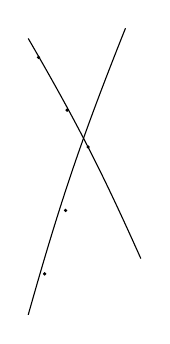
\begin{tikzpicture}[scale=.65]
\draw[thin](-1,2.2)to[bend left=3](1.2,-2.1);\draw[thin](.9,2.4)to[bend right=3](-1,-3.2);
\foreach\p in{(-.8,1.83),(-.24,.8),(.17,.08),(-.27,-1.16),(-.68,-2.4)}\fill\p circle(.035);
\end{tikzpicture}}
\[
\widehat{\mathcal X}_{0,4}^{*}\simeq\deleted{\unsure{\mathbb P^1\times\mathbb P^1}}\unsure{\mathrel{-}}\widehat{\mathcal X}_{0,4}
-\text{les quatre sections }\widetilde\Delta_{\unsure{0|1}}\quad\widetilde\Delta_{\unsure{2|1}}\quad\widetilde\Delta_{\unsure{\infty|3}},\quad\widetilde\Delta
\]
\[
\deleted{\unsure{\widehat{\mathcal X}_{0,\ell}}}\quad\widehat M_{0,5}\quad\text{via}\quad\widehat{\mathcal X}_{0,4}^{*}\ ?
\]
que manque-t-il :

Courbes \inserted{MD} de type $(0,5)$ qui ne sont plus stables en enlevant un des pts à l'infini
\inserted{Il faut que ce soit une \unsure{courbe régulière}}
\figure{\begin{tikzpicture}[scale=.88,every node/.style={font=\small}]
\node at(-.25,.65){$5$};\draw(0,0)--(1.5,0);\draw(0,0)--(-.16,.9);\draw(0,0)--(.2,.9);\draw(1.5,0)--(1.3,.9);\draw(1.5,0)--(1.55,.9);\draw(1.5,0)--(1.9,.8);
\begin{scope}[shift={(1.5,-2.15)}]
\draw(-1,1.65)to[bend right=5](.95,-.6);\draw(.65,1.5)to[bend left=2](-.55,-2.1);
\draw(-.87,1.43)--(-.67,1.27);\draw(-.85,1.26)--(-.67,1.44);
\node[left]at(-.86,1.31){$5$};\fill(-.52,1.03)circle(.04);\node[left]at(-.52,1.03){$i$};
\foreach\p in{(-.22,-1.09),(-.39,-1.57),(-.49,-1.87)}\fill\p circle(.04);
\node at(-1.55,-.2){$1\leq i\leq4$};
\end{scope}
\begin{scope}[shift={(4.7,-1.9)}]
\draw(0,0)--(1.5,.1)--(2.8,.28);\draw(0,0)--(-.18,1.2);\draw(0,0)--(.3,1.25);\draw(1.5,.1)--(1.47,1.25);\draw(2.8,.28)--(2.58,1.5);\draw(2.8,.28)--(3.3,1.5);
\end{scope}
\node at(10,-2.15){$\mathbb P$};
\begin{scope}[shift={(5.6,-4.45)}]
\draw(-1.3,1.65)--(-.28,-.5);\draw(2.9,1.95)to[bend right=3](2.35,-.7);\draw(-1.15,0)to[bend left=4](3.4,.4);
\foreach\p in{(-1.04,1.12),(-.82,.65),(2.82,1.62),(2.7,1.16),(1.08,.22)}\fill\p circle(.04);
\end{scope}
\end{tikzpicture}}
\deleted{$\unsure{\widehat{\mathcal X}}$}
\diagram{\begin{tikzcd}[ampersand replacement=\&, column sep=large,row sep=large]
\widehat X_{0,4}\arrow[d]\&\widehat{\mathcal X}_{0,4}\times\widehat X_{0,4}\arrow[l]\arrow[d,shift right=1]\phantom{.}\\
\deleted{\widehat M_{0,4}}\arrow[r,phantom,"\supset"]\&\widehat{\mathcal X}_{0,4}\arrow[u,bend right=35,"{\sigma_i\ (1\leq i\leq4),\ \delta}"']
\end{tikzcd}}
\figure{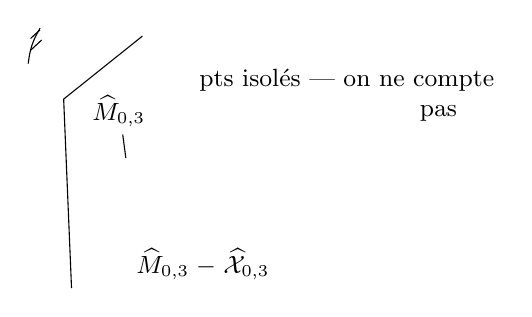
\begin{tikzpicture}[every node/.style={font=\small}]
\draw(-1.2,1.7)--(-2.2,.9)--(-2.1,-1.5);
\node at(-1.5,.75){$\deleted{\widehat M_{0,3}}$};\draw(-1.45,.45)--(-1.41,.15);
\node[anchor=west]at(-1.4,-1.2){$\widehat M_{0,3}\mathrel{-}\widehat{\mathcal X}_{0,3}$};
\node[anchor=west,align=left]at(-.6,.95){\uline{pts isolés} --- on ne compte\\\hspace*{2.8cm}pas};
\draw(-2.5,1.8)to[bend right=12](-2.65,1.35);\draw(-2.62,1.67)--(-2.5,1.78);\draw(-2.62,1.52)--(-2.48,1.65);
\end{tikzpicture}}
\mspage{67}
